% \levelC{Dataset}
This study uses the Govdocs1 dataset \cite{garfinkel_bringing_2009}, which was fully downloaded and its files were grouped by extension. This dataset has files with 63 different extensions. The 33 extensions with less than 200 files were discarded. The  ``text'' and ``unk'' extensions were discarded because files with these extensions use multiple formats and they do not correspond to a single file type. From the remaining 28 extensions, listed in table \ref{tab:govdocs1}, 200 files of each were randomly selected, 100 to use in the training dataset and 100 to use in the validation dataset.

% \levelC{Hardware}
The experiments did not take advantage of GPU acceleration and were  conducted on a single computer with 256GB of RAM and with 2 Intel\textregistered Xeon\textregistered E5-2630 v2 processors, with 6 cores each, with 2 hyper-threads per core, or 24 hyper-threads in total. 


% \levelC{Software}
The main software and frameworks used to build the experiments were Python 3.6, Jupyter notebook, Tensorflow 1.14.0, Keras 2.2.4-tf, and Fedora Linux 27.

% repository
The source code for the experiments is available at \sloppy\url{http://github.com/atilaromero/randomness-experiments}.


% \levelC{Results}
For some file types, training achieved an accuracy higher than 98\% on the first pass. These are the file types where a model should have no difficulty finding patterns. For the remaining file types, all achieved an accuracy higher than 98\% on the second pass, which is fortunate, as this avoids the need to use further passes and  simplifies calculations.

Figure \ref{fig:not_random} shows, for each file type, the percent of 512-byte fragments identified as ``structured'', from a sample of 1000 fragments for each file type.

\noindent
\begin{figure*}[htb!]
\centering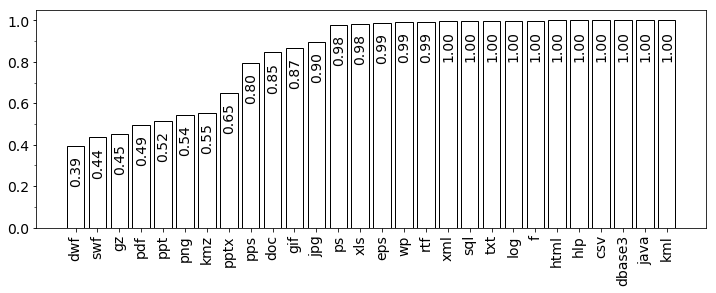
\includegraphics[width=1.0\textwidth]{content/random.png}
\caption{\label{fig:not_random}Validation accuracy of models trained to distinguish each file type from random data. The 90\% accuracy of JPG, for example, means that recognizable patterns were found on 90\% of the blocks of the JPG dataset.}%
\end{figure*}

